% vim:spell:spelllang=en:fo-=a
\chapter{Register Allocation\Author{F. Bouchez \andAuthor S. Hack\andAuthor F. Rastello}}
\label{chapter:register_allocation}
\inputpath{part4}{register_allocation}
\inputprogress

{
  \def\vir{\textrm{in\_regs}}
  \def\vim{\textrm{in\_mem}}
  \def\prot{\textrm{protected}}



\newenvironment{important}{%
\bgroup \color{blue!50!black}
  }{
\egroup 
}

%% Local macros for personal use
% \newcount\todocount \todocount=0
% \def\todo#1{\global\advance\todocount by 1 {\color{blue} {\bf TODO:} #1}}
% \newlinechar=`\^^J
% \def\endofchapter{\ifnum\todocount>0\immediate\write16{^^J! WARNING: There was 
% still TODO macros: \the\todocount.^^J}\fi}


\def\
\def\ac#1{#1}
\def\dom{\preceq}
\def\ssa{SSA\xspace}
\def\maxlive{\ensuremath{\mathrm{Maxlive}}\xspace}
\def\regs{\ensuremath{R}\xspace}
\def\deg{\textrm{degree}\xspace}
\def\irc{Iterated Register Coalescing\xspace}
\newcommand\gr[1]{greedy-$#1$-colorable\xspace}



Register allocation maps the variables of a program to physical memory locations.
The compiler determines the location for each variable and each program point.
Ideally, as many operations as possible should draw their operands from processor registers without loading them from memory beforehand.
Due to the large latency of the memory hierarchy, register allocation is one of the most important optimizations in a compiler. 
As there is only a small number of registers available in a CPU (with usual values ranging from~8 to~128), it is usually not possible to only use registers, and the task of register allocation is also to decide which variables should be evicted from registers and at which program points to store and load them from memory (spilling).

Furthermore, register allocation has to remove spurious copy operations (copy coalescing) inserted by previous phases in the compilation process, and to deal with allocation restrictions that the instruction set architecture and the run-time system impose (register targeting).
Classical register allocation algorithms address those different issues with either complex and sometimes expensive schemes (usually graph-based), or simpler and faster (but less efficient) algorithms such as linear-scan.

The goal of this Chapter is to illustrate how SSA form can help in designing both simpler and faster schemes with similar or even better quality than the most complex existing ones.

\section{Introduction}

Let us first review the basics of register allocation, to help us understand the choices made by graph-based and linear-scan style allocations.

Register allocation is usually performed per procedure. 
In each procedure, a liveness analysis (see Chapter~\ref{chapter:liveness}) determines for each variable the program points where the variable is alive. 
The set of all program points where a variable is alive is called the \emph{live-range} of the variable, and all along this live-range, storage needs to be allocated for that variable, ideally a register. When two variables ``exist'' at the same time, they are conflicting for resources, i.e., they cannot reside in the same location.

This resource conflict of two variables is called \emph{interference} and is usually defined via liveness: 
two variables interfere if (and only if) there exists a program point where they are simultaneously alive, i.e., their live-ranges intersect.%
\footnote{ This definition of interference by liveness is an over-approximation (see Section~\ref{sec:properties_and_flavors:ultimate_interference} of Chapter~\ref{chap:properties_and_flavors}), and there are refined definitions that create less interferences (see Chapter~\ref{chapter:alternative_ssa_destruction_algorithm}). 
  However, in this chapter we will restrict ourselves to this definition and assume that two interfering variables cannot be assigned the same register. 
}
It represents the fact that those two variables cannot share the same register.
For instance, in Figure~\ref{fig:ra:running}, variables $a$ and $b$ interfere 
as $a$ is alive at the definition of $b$.

\subsection{Questions for register allocators}

There are multiple questions that arise at that point that a register allocator has to answer:
\begin{itemize}
  \item Are there enough registers for all my variables? (\emph{spill test})
  \item If yes, how do I choose which register to assign to which variable? (\emph{assignment})
  \item If no, how do I choose which variables to spill to memory? (\emph{spilling})
\end{itemize}

Without going into the details, let us see how linear-scan and graph-based allocators handle these questions.
Figure~\ref{fig:ra:running} will be used in the next paragraphs to illustrate how these allocators work.

\begin{figure}
  % \noindent
  % \begin{center}
    \subfloat[Linear scan]{
      \strut\hspace{-3em}
      \tikzfigure{linear-scan}%
      \label{sub:ra:running-linear}
    }
    \kern-2em
    \subfloat[Graph-based]{%
      \defuseheight{\tikzsubfigure[1]{running}}%
      \label{sub:ra:running-gr}
    }
    \subfloat[Interference graph]{%
      \quad
      \centerheight{\tikzfigure{running-ig}}%
      \label{sub:ra:running-ig}%
    }
  % \end{center}
  \caption{Linear scan makes an over-approximation of live-ranges as
    intervals, while graph-based allocator create an interference graph 
    capturing the exact interferences. Linear scan requires 5 register 
    in this case while coloring the interference graph can be done with 
    4 registers.}
  \label{fig:ra:running}
\end{figure}


\paragraph{Linear-scan} The linear-scan principle is to consider that a procedure is a long basic block and hence live-ranges are approximated as intervals.
For instance, the procedure shown on Figure~\ref{sub:ra:running-gr} is viewed as the straight-line code of Figure~\ref{sub:ra:running-linear}.
The algorithm then proceeds in scanning the block from top to bottom.
When encountering the definition of a variable (i.e., the beginning of a live-range), we check if some registers are free (\emph{spill test}).
If yes, we pick one to assign the variable to (\emph{assignment}). If no, we choose from the set of currently live variables the one that has the farthest use and spill it (\emph{spilling}).
When we encounter the end of its live-range (e.g., a last use), we free the register it was assigned to.

\paragraph{Graph-based}
Graph-based allocators, such as the ``\irc'' allocator (IRC), represent interferences of variables as an undirected \emph{interference graph}: the nodes are the variables of the program, and two nodes are connected if they interfere, i.e., if their live-range intersect.
For instance, Figure~\ref{sub:ra:running-ig} shows the interference graph of the code example presented in Figure \ref{sub:ra:running-gr}.
In this model, two neighbouring nodes must be assigned different registers, so the assignment of variables to registers amounts to \emph{coloring} the graph---two neighbouring nodes must have a different color---using at most $R$ colors, the number of registers.\footnote{Hence the terms ``register'' and ``color'' will be used interchangeably in this chapter.}

Here, the allocator will try to color the graph, if it succeeds (\emph{spill test}), then the coloration represents a valid assignment of registers to variables (\emph{assignment}). If not, the allocator will choose some nodes (usually the ones with the highest number of neighbours) and remove them from the graph by storing the corresponding variables in memory (\emph{spilling}).


\paragraph{Comparison}

Linear-scan is a very fast allocator that works directly on the procedure.
In its model, its spill test is exact and its spill minimizes the amount of loads and store.
However, the model itself is very imprecise as procedures generally are not just straight-line codes but involve complex flow structures such as if-conditions and loops.
In this model, the live-ranges are artificially longer so produce more interferences than there actually are.

On the other hand, a graph-based allocator has a much more precise notion of interference.
Unfortunately, graph $k$-coloring is known to be an NP-complete problem, and the interference graphs of programs are arbitrary.
What causes this are precisely the complex control-flow structure as these creates cycles in the interference graph.
This means the allocator will use heuristics to color, and will base its spill decisions on this heuristic.


Let us look again at the example Figure~\ref{fig:ra:running}, that presents a very 
simple code with an if-condition.
There are two initial variables $a$ and $b$ that end in the branches, and two variables $x$ and $y$ are defined in those branches, as well as a variable $p$ that is always live.
Linear scan would decide it needs five registers (spill test), as the live ranges of all variables are artificially increased: for instance, $a$ is marked alive all along the left branch even though in is never used there.
%
IRC would create the graph on the right, which presents a 4-clique (a complete sub-graph of size 4: with variables $a$, $b$, $p$, and $x$), hence would require at least 4 colors.
This simple graph would actually be easily 4-colorable with a heuristic, hence the spill test would succeed with four registers.

Still, one could remark that at each point of the procedure, only three variables are alive at the same time.
But since $x$ interferes with $b$ on the left branch, and with $a$ on the right branch, it is impossible to use only three registers.

\medskip

In conclusion, linear-scan allocators are faster, and graph coloring ones have better results in practice, but both approaches have an inexact spill test: linear-scan has artificial interferences, and graph coloring uses a coloring heuristic.
Moreover, both require variables to be assigned to \emph{exactly one register} for all their live range.
This means both allocators will potentially spill more variables than strictly necessary, and we will see how SSA can help with this problem.


\begin{figure}
  \begin{center}
    \subfloat[Splitting variable $x$]{%
      \tikzsubfigure[2]{running}
      \label{sub:ra:running-split}
    }
    \subfloat[SSA version]{\tikzsubfigure[3]{running}
      \label{sub:ra:running-SSA}
    }
  \end{center}
  \caption{Splitting variable $x$ in the previous example breaks the 
    interference between $x$ and $a$. Now only 3 registers are required.
    SSA introduces splitting that guarantees \maxlive registers are enough.
  }
  \label{fig:ra:running-split-SSA}
\end{figure}



\subsection{Maxlive and variable splitting}




The number of simultaneously alive variables at a program point is called the \emph{register pressure} at that program point.
%
The maximum register pressure over all program points in a procedure is called the register pressure of that procedure, or ``\maxlive.'' 
One can observe that \maxlive expresses the \emph{minimum} number of required registers for a spill-free register assignment, i.e., an allocation that does not require memory.
For instance, in Figure~\ref{fig:ra:running}, $\maxlive = 3$ so a minimum number of 3 registers is required.
For a straight-line code (basic block), \maxlive constitutes also a \emph{sufficient number of registers}.
% For instance, in Figure~\ref{fig:ra:running}, if the linearized code on the left of Figure~\ref{fig:ra:running} was an actual basic block, it would effectively require exactly four registers.
But in general, a procedure might require \emph{more than \maxlive registers} to be spill-free, indeed, we have seen that the code example actually requires 4 registers, because of the $a,b,p,x$ clique of interferences.




\begin{comment}

Let us see an example in Figure~\ref{fig:ra:linearscan}: in such a case, a greedy assignment considering live intervals from top to bottom always succeeds with \maxlive registers.
In our example, $\maxlive = 2$; Let us assume we have only two registers available (denoted $R_1$ and $R_2$). The greedy algorithm will
assign variable $a$ to $R_1$, then $d$ must be assigned to $R_2$. Finally,
at the definition point of $e$, $R_1$ is released as this is the end of the live-range of $a$, so $e$ can be assigned to $R_1$.
Note that the order of assignment of live-ranges to registers is important.
As an example, a greedy assignment that does not follow the program order could fail, e.g., by assigning $a$ to $R_1$, then $e$ to $R_2$, there is no register available for $d$.


\newsavebox{\linearscanbox}
\begin{lrbox}{\linearscanbox}
  \begin{minipage}{0.55\textwidth}
    \small
\begin{verbatim}
Linear_Scan(B)
  foreach prog point p in B from top to bottom:
    foreach liverange v ending at p
      available[color(v)] = True       
    foreach liverange v starting at p
      c = choose_color(v, available)   
      available[c] = False
      color(v) = c
\end{verbatim}        
\end{minipage}
\end{lrbox}

\begin{figure}
  \subfloat[Example]{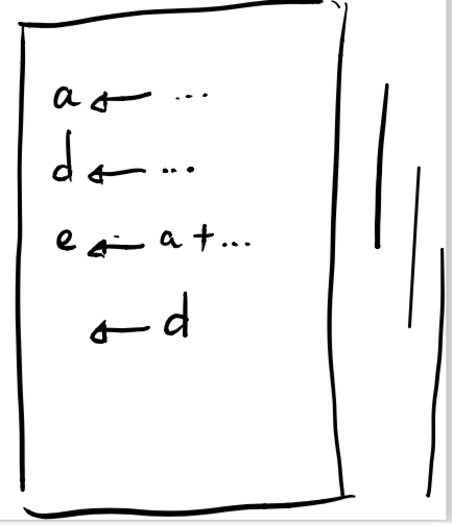
\includegraphics[width=0.27\textwidth]{figures/ra_linearscan.pdf}}
  \hfill
  \subfloat[Linear scan]{\usebox{\linearscanbox}}
  \caption{Linear-scan assignment scheme on a basic block: assigning registers 
  to live intervals from top to bottom ($a$, then $d$, followed by $e$) always 
succeeds if \maxlive (here two) does not exceed the number of available 
registers.}
  \label{fig:ra:linearscan}
\end{figure}



That important observation gave rise to the linear-scan register allocation scheme widely adopted by just-in-time compilers, as the algorithm is very fast.
However, for a general control-flow graph, the algorithm is not optimal, so classical register allocation schemes like to think of interferences as an undirected \emph{interference graph}: the nodes are the variables of the program, and two nodes are connected if they interfere.
A \emph{coloring} of this graph with~$k$ colors corresponds to a valid register allocation with~$k$ registers.\footnote{Hence the terms ``register'' and ``color'' will be used interchangeably in this chapter.}
A $k$-coloring is a mapping from the nodes of the graph to the first~$k$ natural numbers (called colors) such that two neighbouring nodes have different colors.
Unfortunately, graph $k$-coloring is known to be an NP-complete problem, and for any arbitrary undirected graph, there is a program whose interference graph is this graph.
This is the major nuisance of classical register allocation:
the compiler cannot efficiently determine if spilling is necessary,
which means one might need more registers than \maxlive.

The somewhat non intuitive result is that, even if at every program point there are no more than \maxlive variables alive, we still might need more than $\maxlive$ registers for a spill-free register allocation!
The causes of this problem are control-flow merges, as can be seen in Figure~\ref{fig:ra:exprg}.
In that example, the register pressure is at most two at every program point.
However, because the variable $e$ is defined in both branches of an if-condition, the interference graph cannot be colored with two colors: its \emph{chromatic number} is three.
The inequality between \maxlive and the chromatic number is caused by the cycle in the interference graph.


\begin{figure}[htbp]
	\begin{center}
		\subfloat[Example program and live-ranges of its variables]{ 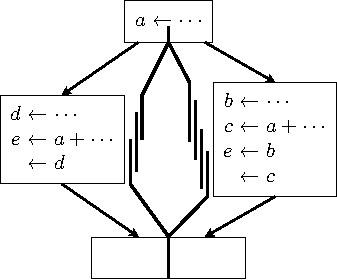
\includegraphics{figures/prog_lr.pdf}
                \label{sub:ra:exprg:prog}
                }
		\qquad
		\subfloat[Interference graph]{ 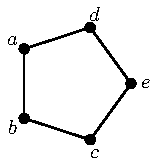
\includegraphics[scale=1.1]{figures/prog_ig.pdf} }
	\end{center}
        \caption{Example program and its interference graph.}
	\label{fig:ra:exprg}
\end{figure}
\end{comment}


This situation changes if we permit \emph{live-range splitting.} 
This means inserting a copy (move) instruction at a program point that creates a new version of a variable. 
Thus, the value of a variable is allowed to reside in different registers at 
different times.  For instance, in Figure~\ref{sub:ra:running-gr}, we 
can split $x$ in the right branch by changing the definition to $x'$ and using 
a copy $x \gets x'$ at the end of the block, producing the code shown on Figure~\ref{sub:ra:running-split}.
It means the node $x$ in the graph is split into two nodes, $x$ and $x'$.
Those nodes don't interfere, and also interfere differently with the other variables:
Now, $x$ can use the same register as $a$ because only $x'$ interferes with $a$.
Conversely, $x'$ can use the same register as $b$, because only $x$ interferes with $b$.
In this version, we only need $\maxlive = 3$ registers, which means that, if the number of registers was tight, we have traded a spill (here one store and one load) for one move, which is an excellent bargain.


This interplay between live-range splitting and colorability is the key issue in register allocation, and we will see in the remainder of this chapter how SSA, which creates live-range splitting at particular locations, can play a role in register allocation.
% (cf.~the SSA version of the program shown in Figure~\ref{fig:ra:exprgssa}). 

% \begin{figure}[htbp]
	% \begin{center}
		% \subfloat[Example program with live-range of~$e$ split]{ 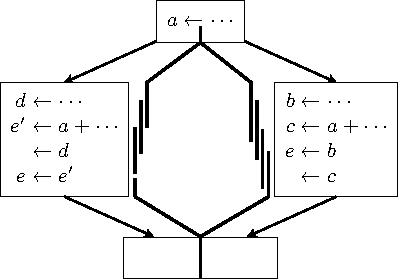
\includegraphics{figures/prog_split_lr.pdf} }
		% \qquad
		% \subfloat[Interference graph]{ 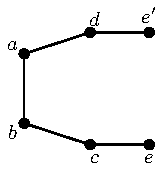
\includegraphics[scale=1.1]{figures/prog_split_ig.pdf} }
	% \end{center}
	% \caption{Example Program with spit live-range and its interference graph}
	% \label{fig:ra:exprgsplit}
% \end{figure}


\subsection{The spill test under SSA}
\label{sec:ra:spilltestssa}

\begin{comment}
As finding a valid $k$-coloring is NP-complete, assigning registers is performed in classical register allocators by some heuristic algorithm.
If that algorithm fails to assign a register to a variable, then it either spills this variable to memory, or frees a register by spilling the variable it contains.
The problem here is that the spilling decision is made to revive the coloring heuristic, and not because the variable that gets spilled is in itself a good candidate for spilling. 
Even worse, we might spill a variable because the heuristic is ``not good enough,'' and not because we are actually out of registers!

In that regard, whatever the coloring heuristic, live-range splitting (up to the extreme setting of splitting at every program point) will never produce ``over-spilling'' decisions.
But if one wants to avoid spill code (memory loads and stores) as much as possible, too many register-to-register copies should also be avoided.
For that purpose, at the same time coloring and spilling decisions are made, classical algorithms also perform copy coalescing (i.e.,~undoing live-range splitting).
However, if done aggressively, coalescing may increase the chromatic number of the graph, or make the graph harder to color for the heuristic.
Thus, existing techniques often apply \emph{conservative} coalescing approaches which are guaranteed not to increase the chromatic number of the graph, at the expense of the quality of the coalescing.
The main issue with conservative coalescing is that, with an extreme solution that would split all live-ranges at every basic block boundaries, it is either slow or inefficient in removing most of the spurious introduced copies.
Thus, the splitting or not splitting trade-off has to be addressed by the register allocator.

We will see that live-range splitting based on SSA form is an elegant solution to this trade-off problem as it is sufficient in bringing the interference graph \maxlive-colorable without blowing-up the number of live-ranges.
\end{comment}

As already mentioned in Section~\ref{sec:properties_and_flavours:domprop} of Chapter~\ref{chapter:properties_and_flavors}, the live-ranges in an SSA form program with dominance property have interesting structural properties:
In that flavor, SSA requires that all uses of a variable are dominated by its definition.
Hence, the whole live-range is dominated by the definition of the variable.
Dominance, however, induces a tree on the control-flow graph.
Thus, the live-ranges of SSA variables are all tree-shaped.
They can branch downwards on the dominance tree but have a single root:
the program point where the variable is defined.
Hence a situation like in Figure~\ref{fig:ra:running} can no longer occur:
$x$ and $y$ had two ``roots'' because they were defined twice.
Under SSA form, the live-ranges of those variables are split by \phifuns, which creates the code shown on Figure~\ref{sub:ra:running-SSA}, where we can see that live-ranges form a ``tree.''
The argument and result variables of the \phifuns constitute new live-ranges, giving more freedom to the register allocator since they can be assigned to different registers.

This structural property is interesting as we can now perform exact polynomial coloring schemes that work both for graph-based and linear-style allocators.


\paragraph{Graph-based} 
Graph-based allocators such as the IRC mentioned above use a \emph{simplification scheme}, that works quite well in practice but is a heuristic for coloring general graphs.
Interestingly, under SSA, the interference graph becomes a chordal graph, which means the simplification scheme will always manage to color the graph with \maxlive colors.
Thus the same classical algorithm can be used without any modification, and now becomes an exact spill test.


\paragraph{Tree-scan (linear-style)}

\begin{algorithm}
  \caption{Tree scan}
  \label{ra:code:assign-tree-scan}

  \KwIn{$T$, program points in order of the dominance tree}
  \KwOut{color, an assignment of live-ranges to registers}

  \Fn{assign\_color ($p$, available)}{

    \ForEach{$v$ last use at $p$}{
      available[color($v$)] $\gets$ \KwTrue\Comment*{colors not used anymore} \label{ra:linecode:assign-tree-scan:clear}
    }
    \ForEach{$v$ defined at $p$}{
      $c \gets$ choose\_color($v$, available)\Comment*{pick one of the available colors} \label{ra:linecode:assign-tree-scan:assign}
      available[$c$] $\gets$ \KwFalse\;
      color($v$) $\gets$ $c$ 
    }

    \ForEach{child $p'$ of $p$}{
      assign\_color($p'$, copy of available)\;
    }
  }

  assign\_color(root(T), [\KwTrue, \KwTrue, ..., \KwTrue])\;
  \Return color
\end{algorithm}



Under SSA, the live-ranges are intervals that can ``branch,'' but never ``join.''
This allows for a simple generalization of the linear-scan mentioned above that we call the \emph{tree-scan},
and always succeeds in coloring the tree-shaped live-ranges with \maxlive colors.
This greedy assignment scans the dominance tree, coloring the variables from the root to the leaves in a top-down order. 
This means the variables are simply colored in the order of their definitions.
This works because branches of the tree are independent, so coloring one will not add constraints on other parts of the tree, contrary to the general non-SSA case where there are cycles.

The pseudo-code of the tree scan is shown in Algorithm~\ref{ra:code:assign-tree-scan}.
Intuitively, when the scanning arrives at the definition of a variable, the only colored variables are ``above'' it and since there is at most $\maxlive-1$ other variables live at the definition, there is always a free color. 

\paragraph{Conclusion}

The direct consequence is that, as opposed to general form programs, and whether we consider graph-based or scan-based allocators, the only case where spilling is required is when $\maxlive > R$, the number of registers.
This allows to decouple spilling from coloring: 
First, lower the register pressure to at most $R$ everywhere in the program; 
Then, color the interference graph with $R$ colors in polynomial time.



  % \caption{Tree scan coloring algorithm for SSA.}
  % \label{code:assign-tree-scan}




\section{Spilling}

We have seen previously that, under SSA, it is easy to decide in polynomial time whether there is enough registers or not, simply by checking if $\maxlive \leq R$, the number of registers.
The goal of this section is to present algorithms that will lower the register pressure when it is too high, i.e., when $\maxlive > R$, by \emph{spilling} (assigning) some variables to memory.

Spilling has a different meaning depending on the type of allocator used.
For a scan-based allocator, the spilling decision happens when we are at a particular program point.
Although it is actually a bit more complex, the idea when spilling a variable $v$ is that we insert a store at that point, and a load just before its next use, hence we are spilling only a part of the live-range.
%
On the other end, a graph-based allocator has no notion of program points since the interferences have been combined in an abstract structure: the interference graph.
In the graph-coloring setting, spilling means removing a node of the interference graph and thus the \emph{entire} live-range of a variable.
This is a called a \emph{spill everywhere} strategy, which implies inserting load instructions in front of every use and store instructions after each definition of the (non-SSA) variables.
These loads and stores require temporary variables that were not present in the initial graph.
Those variables also need to be assigned to registers, which means that whenever the spilling/coloring is done, the interference graph is rebuilt and a new pass of allocation is triggered, until no variable is spilled anymore: this is where the ``Iterated'' comes from in the IRC name.
In practice, a post-pass of a graph coloring scheme scans each basic block separately, so as to, whenever possible, keep a reloaded variable in a register between multiple uses.

\smallskip

In this section, we will consider the two approaches: the graph-based approach with a spill-everywhere scheme, and scan-based approach that allows partial live-range spilling.
%
In both cases, we will assume that the program was in SSA before spilling. 
This is important to notice that there are pros and cons of assuming so. 
In particular, the inability to coalesce or move the shuffle code associated to \phifuns can lead to spurious load and store instructions on CFG-edges.
Luckily, these can be handled by a post-pass of partial redundancy elimination (PRE, see Chapter~\ref{todo}), and we will consider here the spilling phase as a full-fledged SSA program transformation.

\medskip

Suppose we have $R$ registers, the objective is to establish $\maxlive\le\regs$ (\maxlive lowering) by inserting loads and stores into the program. 
Indeed, as stated above, lowering \maxlive to~\regs ensures that a register allocation with \regs registers can be found in polynomial time for SSA programs. 
Thus, spilling should take place before registers are assigned \emph{and} yield a program in SSA form. 
In such a decoupled register-allocation scheme, the spilling phase is an optimization problem for which we define the following constraints and objective function:
\begin{itemize}
  \item the \emph{constraints} that describe the universe of possible solutions expresses that the resulting code should be \regs-colorable; 
  \item the \emph{objective function} expresses the fact that the (weighted) amount of inserted loads and stores should be minimized.
\end{itemize}

The constraints directly reflect the ``spill test'' which expresses whether more spilling necessary or not.
The objective is expressed with the profitability test: 
among all variables, which one is more profitable to spill? 
The main implication of spilling in SSA programs is that the spill test---which amounts to checking whether \maxlive has been lowered to \regs or not---becomes precise. 

The other related implication of the use of SSA form follows from this observation: 
consider a variable such that for any program point in its entire live-range the register pressure is at most \regs, then spilling this variable is useless with regard to the colorability of the code.
In other words, spilling such a variable will never be profitable. 
We will call this yes-or-no criteria, enabled by the use of SSA form, the ``usefulness test.''


We will see now how to choose, among all ``useful'' variables (with regard to the colorability), the ones that seem most profitable.
In this regard, we present in the next section how SSA allows to better account for the program structure in the spilling decision even in a graph-based allocators, thanks to the enabled capability to decouple spilling  (allocation) to coloring (assignment).
However, register allocation under SSA shines the most in a scan-based setting, and we present guidelines to help the spill decisions in such a scheme in Section~\ref{sec:ra:spill-scan}.


\subsection{Graph-based approach}


In a graph-based allocator such as the IRC, a \emph{spill everywhere} strategy is used, a variable is either spilled completely or not at all, and loads are placed directly in front of uses and stores directly after the definition.
When spilled, the live-range of a variable then degenerates into small intervals: one from the definition and the store, and one from each load to its subsequent use.
However, even in this simplistic setting, it is NP-complete to find the minimum number of nodes to establish $\maxlive\le\regs$.
% It is even NP-complete to find the minimum number of nodes to spill to decrease \maxlive just by one!
Variables (graph nodes) are spilled greedily using a weight that takes into account its node degree (number of interfering uncolored variables) and an estimated spill cost (estimated execution frequency of inserted loads and stores).
Good candidates are high-degree nodes of low spill cost, as this means they will lessen coloring constraints on many nodes---their neighbours---while inserting few spill code.

The node degree represents the profitability of spilling the node in terms of colorability.
It is not very precise as it is only a graph property, independent of the control-flow graph.
We can improve this criteria by using SSA to add a usefulness tag.
We will now show how to build this criteria, and how to update it.

\paragraph{Building the ``useful'' criteria}

We attach to each variable $v$ a ``useful'' tag, an integer representing the number of program points that would benefit from spilling $v$, i.e., $v.\textit{useful}$ expresses the number of program points that belong to the live-range of $v$ and for which the register pressure is strictly greater than \regs.
This information can be built at the same time as the interference graph.

Under SSA, the interference graph is built through a simple \emph{bottom-up traversal} of the CFG.
When encountering the last use of a variable $p$, $p$ is added to the set of currently live variables (live-set) and a corresponding node (that we also call $p$) is added in the graph.
Arriving at the definition of $p$, it is removed from the current live-set, and we add edges (interferences) to the graph:
for all variable $v$ in the live-set, there is an edge $(v\to p)$.
Note that, as opposed to standard interference graphs, we consider directed edges here, where the direction represents the dominance.
At that point, we also associate the following fields to node $p$ and its interferences: 
\begin{itemize}
  \item $p.\textit{pressure}$, that corresponds to the number of variable alive at the definition point of $p$, i.e., $|\textrm{live-set}| + 1$;
  \item $(v\to p).\textit{high}$, a boolean set to \true if and only if $p.\textit{pressure}>\regs$, meaning this interference belongs to a clique of size more than $R$.
\end{itemize}

We then create the ``usefulness'' field of $p$. If $p.\textit{pressure} \leq \regs$, then $p.\textit{useful}$ is set to 0. Otherwise, we do the following:
\begin{itemize}
  \item $p.\textit{useful}$ is set to 1;
  \item for all $(v\to p)$, $v.\textit{useful}$ gets incremented by 1.
\end{itemize}

At the end of the build process, $v.\textit{useful}$ expresses the number of program points that belong to the live-range of $v.\textit{var}$ and for which the register pressure is greater than \regs. 
More precisely,
%
$$v.\textit{useful}=\left|\lbrace p : (v\to p)\ \textrm{exists}\; \wedge\; p.\textit{pressure}>\regs  \rbrace\right|$$

With this definition, if $v.\textit{useful}=0$, then it can be considered to be be useless to spill $v$, as it will not help in reducing the register pressure.
If not, it means that $v$ belongs to this number of cliques of size greater than $\regs$.
Since at least one of the nodes of those cliques must be spilled, spilling $v$ is useful as it would reduce the size of each of those cliques by one.
Existing coloring scheme such as the IRC can be modified to use the \emph{useful} tag when making spill decisions, the higher the better.


\paragraph{Updating the ``useful'' criteria}


Whenever a node $n$ is spilled (assume only useful nodes are spilled), those additional fields of the interference graph must be updated as follows:
\begin{enumerate}
  \item if $n.\textit{pressure}>\regs$, for all its incoming edges $(v\to n)$, $v.\textit{useful}$ is decremented by one;
  \item for all its successors $p$ such that $(n\to p).\textit{high} = \textrm{True}$, $p.\textit{pressure}$ is decremented by one; if, following this decrement, $p.\textit{pressure} \leq \regs$, then for all the incoming edges $(v,p)$ of $p$, $v.\textit{useful}$ is decremented by one.
\end{enumerate}


\paragraph{Thoughts on graph-based spilling}

In an existing graph-based allocation, SSA can bring information to better help the allocator in making its spill decisions.
However, with the spilling and coloring fully decoupled, encoding the information using a graph does not seem as pertinent.
Moreover, formulations like \emph{spill everywhere} are often not appropriate for practical purposes, as putting the whole live-range to memory is too simplistic. 
A variable might be spilled because at some program point the pressure is too high, however, if that same variable is later used in a loop where the register pressure is low, a spill everywhere will place a superfluous (and costly!) load in that loop. 
Spill everywhere approaches try to minimize this behavior by adding costs to variables, to make the spilling of such a variable less likely.
These bring in a flow-insensitive information that a variable reside in a frequently executed area, but such approximations are often too coarse to give good performances.
Hence, it is imperative to cleverly split the live-range of the variable according to the \emph{program structure} and spill only parts of it, which is why we prefer to recommend a scan-based approach of the register allocation under SSA.


\subsection{Scan-based approach}% (a.k.a. ``Tree-scan'')}
\label{sec:ra:spill-scan}


In the context of a basic block, a simple algorithm that works well is the ``furthest first'' algorithm that is presented in Algorithm~\ref{ra:code:ff}.
The idea is to scan the block from top to bottom:
whenever the register pressure is too high, we will spill the variable whose next use is the furthest away, and it is spilled only \emph{up to this next use}.
In the \textit{evict} function of Algorithm~\ref{ra:code:ff}, this correspond to maximizing \textrm{distance\_to\_next\_use\_after($p$)}.
%
Spilling this variable frees a register for the longest time, hence diminishing the chances to have to spill other variables later.
This algorithm is not optimal because it does not take into account the fact that the first time we spill a variable is more costly than subsequent spills of the same variable (the first time, a store and a load are added, but only a load must be added afterwards).
However, the general problem is NP-complete, and this heuristic, although it may produce more stores than necessary%
%(e.g., by spilling two variables while spilling an other part of the first one would have been enough)
, gives good results on ``straight-line codes,'' i.e., basic blocks.

\begin{algorithm}[h]
  \caption{Furthest First spilling algorithm for straight-line code}
  \label{ra:code:ff}

  \KwIn{$B$, the basic block to process}
  \KwIn{\vir, the set of variables in registers at entry of $B$}
  % \KwOut{color, an assignment of live-ranges to registers}

% \_First ($B$: basic block, var\_in\_regs)}{


  \ForEach{program point $p$ in $B$ from top to bottom}{
    \Comment{uses of $v$ must be in a register before $p$}
    $\prot \gets \emptyset$\;
    \ForEach{$v$ used at $p$}{
      \If{$v \notin \vir$}{
          insert a load of $v$ from memory just before $p$\;
          add $v$ to \vir\;
          add $v$ to \prot\;
          %$\vir \gets \vir \cup \{v\}$\;
      }
    }

    evict($p$, \vir, \vim, \prot)
    \Comment*{need space for vars loaded at $p$}

    \ForEach{$v$ last use at $p$}{
      remove $v$ from \vir\;
    }
    $\prot \gets \emptyset$\;
    \ForEach{$v$ defined at $p$}{
      add $v$ to \vir\;
      add $v$ to \prot\;
    }
    evict($p$, \vir, \vim, \prot) \Comment*{need space for vars defined at $p$}
  }


  \Fn{evict ($p$, \vir, \vim, \prot)}{
    \Comment{remove variables from registers until there are enough registers}
    \While{$| \vir | > R$}{
      let $v \in (\vir \setminus \prot)$ with maximum $v$.distance\_to\_next\_use\_after($p$)\;
      \If{$v \notin \vim$}{
         insert a store of $v$ to memory just before $p$\;
         add $v$ to \vim\;
       }
       remove $v$ from \vir\;
    }
  }
\end{algorithm}

\medskip

We now present an algorithm that extends this ``furthest first'' algorithm to general control-flow graphs.
The idea is to scan the CFG using a topological order and greedily evict sub live-ranges whenever the register pressure is too high.
There are two main issues:
\begin{enumerate}
  \item Generalize the priority function distance\_to\_next\_use\_after to a general CFG;
  \item Find a way to initialize the ``in\_regs'' set when starting to scan a basic block, in the situation where predecessor basic blocks have not been processed yet (e.g., at the entry of a loop).
\end{enumerate}


\paragraph{Profitability to Spill}
To illustrate the generalization of the further-first priority strategy to a CFG, let us consider the example of Figure~\ref{fig:ra:priority-spill-CFG}.
In this figure, the $\lightning +n$ sign denotes regions with (high) register pressure of $\regs+n$.
At program point $p_0$, register pressure is too high by one variable (suppose there are other hidden variables that we do not want to spill).
We have two candidates for spilling: $x$ and $y$, and the classical furthest first criteria would depend on which branch is chosen:

\begin{itemize}
  \item If the left branch is taken, and consider the execution trace ($AB^{100}C$).
  In this branch, the next use of $y$ appears in a loop, while the next use of $x$ appears way further, after the loop has fully executed. 
  It is clearly considered to be more profitable to evict variable $x$ (at distance 101).

  % Looking at this execution trace in isolation, and using the further first strategy described above for straight-line code

\item If the right branch is taken, and consider the execution trace ($AD$).
  In that case, this is variable $y$ has the further use (at distance 2) so we would evict variable $y$.

\end{itemize}

Looking at the example as a whole, we see that the left branch is not under pressure, so spilling $x$ would only help for program point $p_0$, and one would need to spill another variable in block $D$ ($x$ is used at the beginning of $D$), hence it would be preferable to evict variable $y$.

On the other hand, modifying a little bit the example by assuming a high register pressure within the loop at program point $p_1$ (by introducing other variables), then evicting variable $x$ would be preferred in order to avoid a load and store in a loop!

% \bigskip


This dictates the following remarks:
\begin{enumerate}
  \item Program points with low register pressure can be ignored.
  \item Program points within loops, or more generally with higher execution frequency should account in the computation of the ``distance'' more than program points with lower execution frequency.
\end{enumerate}

\begin{figure}
  \todo{ add variable 'a' defined after 'y' and used everywhere, and set R = 2)
  => or better : explain there are other code not shown, but for pedagogical purposes we know the pressure and want only to spill x or y.
  There should be a use of $y$ in the loop, no ?! Remove also $z$.
}
  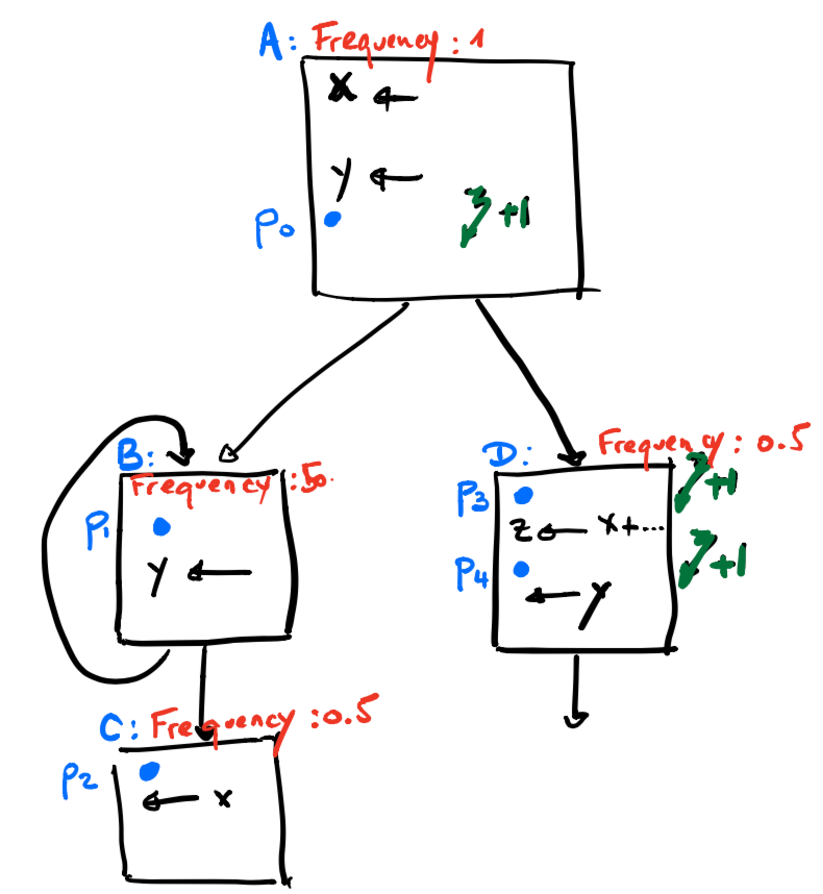
\includegraphics[width=0.45\textwidth]{figures/priority-spill-CFG.pdf}

  \caption{Generalization of \texttt{distance\_to\_next\_use\_after} for a CFG. Illustrating example.}
  \label{fig:ra:priority-spill-CFG}
\end{figure}

So we will replace the notion of ``distance'' in the furthest first algorithm with a notion of ``profitability,'' i.e., a measure of the number of program points (weighted by frequency) that would benefit from the spilling of a variable $v$.

%
% This leads, for a variable $v$ live at program point $p$ to the following definition of function \verb+v.spill_profitability(p)+ where $q.\texttt{frequency}$ represents the estimated execution frequency for a program point $q$:
%

\begin{definition}[Spill profitability from $p$]
%
  Let $p$ be a program point and $v$ a variable live at $p$.
  Let $v.\texttt{HP}(p)$ (High-Pressure) be the set of all program points $q$ such that:
  1.~register pressure at $q$ is strictly greater than \regs;
  2.~$v$ is alive at $q$;
  3.~there exists a path from $p$ to $q$ that does not contain any use or definition of $v$.
  Then,

  $$\texttt{v.spill\_profitability}(p) = \sum_{q\in v.\texttt{HP}(p)} q.\texttt{frequency}$$
  % where
  % $$v\texttt{HP}(p) = \{ q \in live-range(v) | q.pressure > R and q reachable from p \}$$
\end{definition}

There is a important subtlety concerning the set of points in $v.\texttt{HP}(p)$, that is dependent on the instruction set architecture and the way spill code is inserted.
Consider in our example the set $x.\texttt{HP}(p_0)$, i.e., the set of high-pressure points that would benefit from the spilling of $x$ at point $p_0$.
The question is the following: `` does the point $p_3$ (just before the instruction using $x$) belong to this set?''
If the architecture can have an operand in memory, $p_3$ belongs to the set;
However, if the architecture requires an operand to be loaded in a register before its use, then $x$ would be reloaded at $p_3$ so this point would not benefit from the spilling of $x$ and $p_3$ must be excluded from $x.\texttt{HP}(p_0)$.

Let us see how the profitability applies to our running example with two scenarios: low-pressure and high-pressure in the $B$ loop.

\begin{center}
  \begin{tabular}{r@{\quad}cc}
  Loop $B$ & Low-pressure & High-pressure \\
  \hline
  $x.\texttt{HP}(p_0)$ & $\{p_0\}$ & $\{p_0,p_1\}$ \\
  $y.\texttt{HP}(p_0)$ & $\{p_0,p_3\}$ & $\{p_0,p_3\}$ \\
  $x.\texttt{spill\_profitability}(p_0)$ & $1$ & $51$ \\
  $y.\texttt{spill\_profitability}(p_0)$ & $1.5$ & $1.5$ \\
\end{tabular}
\end{center}

In the first case, we would evict $y$, in the second, we would evict $x$ (plus another variable later, when arriving at $p_3$), which is the behaviour we wanted in the first place.

\paragraph{Initial Register Filling at the Beginning of a Basic Block}
For each visited basic block $B$, the set of variables that must reside in a register is stored in $B.\vir$.
For each basic block, the initial value of this set has to be computed before we start processing it.
The heuristic for computing this set is different for a ``regular'' basic block and for a loop entry.
For a regular basic block, as we assume a topological order traversal of the CFG, all its predecessors will have been processed.
Live-in variables fall into three sets:
\begin{enumerate}
\item The ones that are available in all predecessor basic blocks:
  $$B.\textrm{allpreds\_in\_regs}=\bigcap_{P\in \textrm{pred}(B)} P.\vir$$
\item The ones that are available in some of the predecessor basic blocks:
  $$B.\textrm{somepreds\_in\_regs}=\bigcup_{P\in \textrm{pred}(B)} P.\vir$$
\item The ones that are available in none of them.
\end{enumerate}

As detailed in Algorithm~\ref{ra:code:initnormal}, $B.\vir$ is initialized with $B.\texttt{allpreds\_in\_regs}$ plus, as space allows, elements of $B.\texttt{somepreds\_in\_regs}$ sorted in decreasing order of their \texttt{spill\_profitability} metric.
\todo{need to mention that we load them somewhere also : at beginning of block or on edges or end of previous blocks ? : put a comment in algo ?}


\begin{algorithm}[h]
\caption{Initial value of $B.\vir$ for a regular basic block}
\label{ra:code:initnormal}
  \KwIn{$B$, the basic block to process}

  $\textrm{allpreds\_in\_regs} \gets \bigcap_{P\in \textrm{pred}(B)} P.\vir$\;
  $\textrm{somepreds\_in\_regs} \gets \bigcup_{P\in \textrm{pred}(B)} P.\vir$\;

  $B.\vir \gets \textrm{allpreds\_in\_regs}$\;
  \While{$|B.\vir| < R$ and $|\textrm{somepreds\_in\_regs}| > |B.\vir|$}{
    let $v \in (\textrm{somepreds\_in\_regs} \setminus B.\vir)$ with mininum $v$.spill\_profitability($B$.entry)\;
    add $v$ to $B$.\vir\;
  }
\end{algorithm}


\begin{figure}
  \begin{center}
    \subfloat[\label{sub:ra:loopentry_example_a}\vir\ at $B$'s entry]{\qquad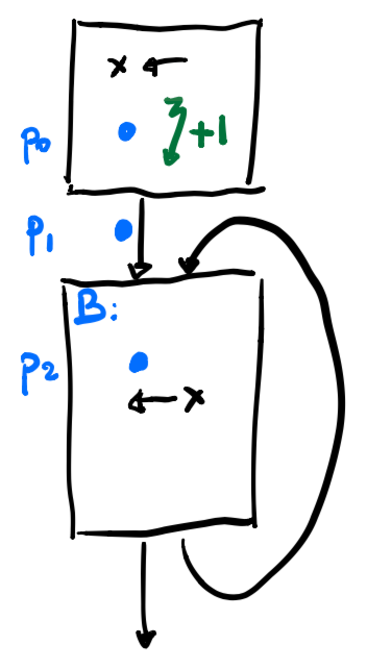
\includegraphics[width=0.15\textwidth]{figures/loopentry_example_a.pdf}\qquad}
    \hfil
    \subfloat[\label{sub:ra:loopentry_example_b}not \vir\ at $B$'s entry]{\qquad\quad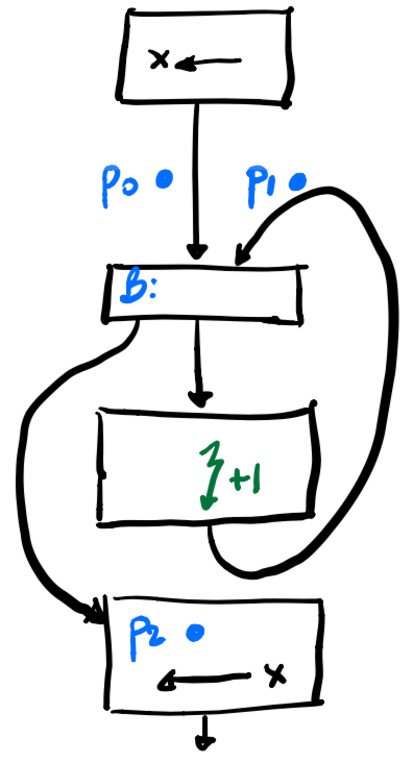
\includegraphics[width=0.15\textwidth]{figures/loopentry_example_b.pdf}\qquad\quad}
  \end{center}
  \caption{\label{fig:ra:loopentry_example}Initial values of $B.\vir$ at loop entry. Illustrating examples.}
\end{figure}
For a basic block at the entry of a loop, as illustrated by the example of Figure~\ref{fig:ra:loopentry_example}, one do not want to account for allocation on predecessor basic block, but start from scratch instead.
Assume the first basic block has already been processed and one wants to compute $B.\vir$:
\begin{enumerate}
  \item Example~\subref{sub:ra:loopentry_example_a}: 
  even if at the end of the predecessor basic block, $x$ is not available in a register, one wants to insert a reload of $x$ at $p_1$, i.e., include $x$ in $B.\vir$.
  Not doing so would involve a reload at every iteration of the loop at $p_2$. 
\item Example~\subref{sub:ra:loopentry_example_b}: 
  Even if at the entry of the loop, $x$ is available in a register, one wants to spill it and restore at $p_2$ so as to lower the register pressure that is too high within the loop.
  This means excluding $x$ from $B.\vir$.
\end{enumerate}
This leads to Algorithm~\ref{ra:code:initloop} where $B.\texttt{livein}$ represents the set of live-in variables of $B$ and $L.\maxlive$ is the maximal register pressure in the whole loop $L$.
\texttt{Init\_inregs} first fills $B.\texttt{in\_regs}$ with live-in variables that are used within the loop $L$.
Then, we fill with live-through variables, but only those that can survive the loop:
if $L.\maxlive>\regs$, then  $L.\maxlive-\regs$ variables will have to be spilled (hopefully some live-through variables);
so no more than $|B.\texttt{livein}|-(L.\maxlive-\regs)$ are allocated to a register at the entry of $B$.

\begin{algorithm}[h]
\caption{\label{ra:code:initloop}Initial value of $B.\vir$ at the entry of a loop $L$}
% Init_inregs(B,L)
  $B.\vir \gets \emptyset$\;
  \While{\\
        \begin{tabular}{@{\hspace*{1.5em}}l@{}}
    $|B.\vir| < R$ \quad and \\
    $|B.\textrm{livein}| > |B.\vir|$ \quad and\\
    $|B.\vir| < R + |B.\textrm{livein}| - L.\maxlive$
      \end{tabular}\\}
    {
    let $v \in (B.\textrm{livein} \setminus B.\vir)$ with minimum $v$.spill\_profitability($B$.entry)\;
    add $v$ to $B.\vir$\;
  }
\end{algorithm}


\paragraph{Putting all Together}
The overall algorithm for spilling comprises several phases:
First, we pre-compute both liveness and profitability metrics;
Then we traverse the CCFG in topological order, and each basic block is scanned using initial value of $B.\vir$ as explained above.
During this phase, we maintain the sets of live-variables available in register and in memory at basic block boundaries.
The last phase of the algorithms handles the insertion of shuffle code (loads and store) where need.
\todo{ref to other chapter, note somewhere ? (see previous todo also)}


\section{Coloring and coalescing}

We advocate here a decoupled register allocation: First, lower the register pressure so that $\maxlive \leq \regs$; Second, assign variable to registers.
Live-range splitting ensures that, after the first phase is done, no more spilling will be required as \regs will be sufficient, possibly at the cost of inserting register-to-register copies.
This is practical for instance when working on an existing compiler that uses a classical register allocation algorithm, for instance, the IRC.


For instance, a solution could be to insert a copy for every variable at every basic block boundary, then linear scan would be able to color each basic block independently. However, this would add a lot of copies.

Minimal SSA form (see Chapter~\ref{chapter:properties_and_flavors}) has this nice property for us that it provides sufficient live-range splitting: the insertion of \phifuns effectively splits variable just enough so that a greedy tree-scan coloring scheme can assign variable to register without more spilling.


We already mentioned in Section~\ref{sec:ra:spilltestssa} that the well-known ``Iterated Register Coalescing'' (IRC) allocation scheme, which uses a simplification scheme can take advantage of the SSA form property.
We will show here that, indeed, the underlying structural property makes a graph coloring simplification scheme (recalled below) an ``optimal'' scheme.
This is especially important because, besides minimizing the amount of spill code, the second objective of register allocation is to perform a ``good coalescing,'' i.e., try to minimize the amount of register-to-register copies:
a decoupled approach is practically viable if the coalescing phase is effective in merging most of the live-ranges, introduced by the splitting from SSA, by assigning live-ranges linked by copies to the same register.

In this section, we will first present the traditional graph coloring heuristic, based on a simplification scheme, and show how it successfully colors programs under SSA form.
We will then explain in greater details the purpose of coalescing, and how it translates when performed on SSA form program.
Finally we will show how to extend the graph-based (from IRC) and the scan-based (of Algorithm~\ref{ra:code:assign-tree-scan}) greedy coloring schemes to perform efficient coalescing.


\subsection{Greedy coloring scheme}
\label{sec:ra:greedy-col}

In traditional graph coloring register allocation algorithms, the assignment of registers to variables is done by coloring the interference graph using a greedy heuristic called a \emph{simplification scheme}.
This scheme is based on the observation that, given \regs colors---representing the registers---, if a node in the graph has at most $\regs-1$ neighbors, there will always be one color available for this node whatever colors the remaining nodes have.
Such a node can be \emph{simplified},\index{simplify} i.e., removed from the graph and placed on a stack.
This process can be iterated with the remaining nodes, whose degree may have decreased (if the simplified node was one of their neighbors).
If the graph becomes empty, we know it is possible to color the graph with \regs colors, by assigning colors to nodes in the reverse order of their simplification, i.e., popping nodes from the stack and assigning them one available color.
This is always possible since they have at most $\regs-1$ colored neighbors.
We call the whole process the \emph{greedy coloring scheme}\index{greedy coloring scheme}:
Its first phase, whose goal is to eliminate nodes from the graph to create the stack is presented in Algorithm~\ref{ra:code:is-k-greedy}, while the second phase, which assigns variables to registers, is presented in Algorithm~\ref{ra:code:assign-color}.


\begin{algorithm}[h]
  \caption{Greedy simplification scheme used by the greedy coloring scheme to create the stack. If this stage succeeds, the graph is said to be \gr{\regs}.}
\label{ra:code:is-k-greedy}
% Function Simplify(G)
\KwIn{$G = (V,E)$ an undirected graph}
\KwIn{$\regs$: number of colors (registers)}
\KwIn{For each vertex $v$, degree[$v$], the number of neighbours in $G$}

\Fn{Simplify(G)}{
  stack $\gets \emptyset$ \;
  worklist $\gets \{v \in V \mid \deg[v] < \regs\}$\;
  \While{worklist $\neq \emptyset$}{
    let $v \in $ worklist \;
    \ForEach{$w$ neighbour of $v$}{
      degree[$w$] $\gets$ degree[$w$]$-1$\;
      \If{degree[$w$] = $\regs - 1$}{ 
        add $w$ to worklist\;
      }
      push $v$ on stack\;
      remove $v$ from worklist\;
      remove $v$ from $V$\Comment*{Remove $v$ from the graph}
    }
  }
  \If{$V \neq \emptyset$}{
    Failure ``The graph is not simplifiable''
  }
  \Return stack\;
}
\end{algorithm}


\begin{algorithm}[h]
\caption{Greedy coloring assignment used in the greedy coloring scheme. The stack is the output of the Simplify function described in Algorithm~\ref{ra:code:is-k-greedy}.}
\label{ra:code:assign-color}
\Fn{Assign\_colors($G$)}{
  available $\gets$ new array of size \regs, with initialized values to \KwTrue\;
  \While{stack $\neq \emptyset$}{
    $v \gets $ pop stack \;
    \ForEach{neighbor $w$ in $G$}{
      available[color($w$)] $\gets$ \KwFalse\Comment*{color already used by neighbor}
    }
    % col $\gets 0$\;
    \ForEach{color $c$}{% from $1$ to \regs}{
      \If{available[$c$]}{
        col $\gets c$\;
      }
      available[$c$] = \KwTrue\Comment*{prepare for next round}
    }
    color($v$) $\gets$ col\;
    add $v$ to $G$\;
  }
}
\end{algorithm}



The greedy scheme is a coloring heuristic for general graphs, and as such, it can get stuck;
it happens whenever all remaining nodes have degree at least \regs.
In that case, we do not know whether the graph is \regs-colorable or not.
In traditional register allocation, this is the trigger for spilling some variables so as to unstuck the simplification process.
However, under the SSA form, if spilling has already been done so that the maximum register pressure is at most \regs, the greedy coloring scheme can never get stuck!
We will not formally prove this fact here but will nevertheless try to give insight as to why this is true.


The key to understanding that property is to picture the dominance-tree, with live-ranges are sub-trees of this tree, such as the one on Figure~\ref{sub:ra:running-SSA}.
At the end of each dangling branch there is a ``leaf'' variable: the one that is defined last in this branch.
These are the variables $y_1$, $y_2$, $y_3$ and $x_3$ on Figure~\ref{sub:ra:running-SSA}.
We can visually see that this variable will not have many intersecting variables:
those are the variables alive at its definition point, i.e., no more than $\maxlive-1$, hence less that $\regs-1$.
On Figure~\ref{sub:ra:running-SSA}, with $\maxlive = 3$ we see that each of them has no more than two neighbors.

Considering again the greedy scheme, this means each of them is a candidate for simplification.
Once removed, another variable will become the new leaf of that particular branch (e.g., $x_1$ if $y_1$ is simplified).
This means simplification can always happens at the end of the branches of the dominance tree, and the simplification process can progress upwards until the whole tree is simplified.

\smallskip

In terms of graph theory, the general problem is knowing whether a graph is $k$-colorable or not.
Here, we can define a new class of graph that contains the graphs colorable with this simplification scheme.
\begin{definition}
  A graph is \gr{k} if it can be simplified using the simplify function of Algorithm \ref{ra:code:is-k-greedy}.\index{\gr{k}}
\end{definition}

\noindent
We then have the following theorem:
\begin{theorem}
Setting $k=\maxlive$, the interference graph of a code under SSA form is always \gr{k}.
\end{theorem}

This tells us that, if we are under SSA form and the spilling has already been done so that $\maxlive \leq R$, the classical greedy coloring scheme is \emph{guaranteed} to perform register allocation with \regs colors without any additional spilling, as the graph is \gr{R}.%
\footnote{Observe that, with a program originally under SSA form, practical implementation may still chose to interleave the process of spilling and coalescing/coloring. Result will be unchanged but speed might be impacted: the important is the \emph{idea} of having a coalescing/coloring phase that will not produce more spilling.}



\subsection{Coalescing under SSA form}
The goal of \emph{coalescing}\index{coalescing} is to minimize the number of register-to-register \emph{move}\index{move instruction} instructions in the final code.
In a graph-based allocation approach where the color everywhere strategy is applied,
each node of the interference graph corresponds to a unique variable which will be allocated to a register along its entire live-range.
%
Coalescing two nodes, or by extension coalescing the two corresponding variables, means merging the nodes in the graph, thus imposing allocating the same register to those variables.
Any copy instruction between those two variables becomes useless and can be safely removed.

This way, coalescing, when done during the register allocation phase, is used to minimize the amount of register-to-register move in the final code.
While there may not be so many such copies at the high-level (e.g., instructions ``$a \gets b$'')---especially after a phase of copy propagation under SSA (see Chapter~\ref{constant_propagation_is_easier})---, many such instructions are added in different compiler phases by the time compilation reaches the register allocation phase. 
For instance, adding copies is a common way to deal with register constraints (see the practical discussion in Section~\ref{sec:practical-regalloc}).

An even more obvious and unavoidable reason in our case is the presence of \phifuns due to the SSA form:
The semantic of a \phifun corresponds to parallel copies on incoming edges of basic blocks, and destructing SSA i.e., getting rid of \phifuns that are not machine instructions, is done through the insertion of copy instructions. 
It is thus better to assign variables linked by a \phifun to the same register, so as to ``remove'' the associated copies between subscripts of the same variable.
As already formalized (see Section~\ref{sec:destruct:quality} of Chapter~\ref{chap:alternative_ssa_destruction_algorithm}) for the aggressive coalescing scheme, we define a notion of \emph{affinity}, acting as the converse of the relation of interference and expressing how much two variables ``want'' to share the same register. 
By adding a metric to this notion, it measures the benefit one could get if the two variables were assigned to the same register: 
the weight represents how many instructions we would save at execution if the two variables share the same register. 
%% For instance, given two variables $a$ and $b$, the weight of the affinity between them is the number of occurrence of copy instructions involving them ($a\gets b$ or $b\gets a$) or \phifuns ($a\gets\phi(\ldots,b,\ldots)$ or $b\gets\phi(\ldots,a,\ldots)$). 
%% Actually, some parts of the program are more often executed than others, and a more accurate cost for each copy can be calculated using actual execution frequencies based on profiling; 
%% It is also possible to use empirical parameters, for instance $\times 10$ for each level of nested loop, $\times 0.5$ if in a conditional branch, etc.


\subsection{Graph-based approach}
Coalescing comes with several flavors, which can be either aggressive or conservative.
Aggressively coalescing an interference graph, means coalescing non-interfering nodes (i.e., constraining the coloring) regardless of the chromatic number of the resulting graph.
An aggressive coalescing scheme is presented in Chapter~\ref{chap:alternative_ssa_destruction_algorithm}.
Conservatively coalescing an interference graph, means coalescing non-interfering nodes without increasing the chromatic number of the graph.
In both cases, the objective function is the maximization of satisfied affinities, i.e., the maximization of the number of (weighted) affinities between nodes that have been coalesced together.
In the current context, we will focus on the conservative scheme, as we do not want more spilling.

Obviously, because of the reducibility to graph-$k$-coloring, both coalescing problems are NP-complete.
However, graph coloring heuristics such as the \irc use incremental coalescing schemes where affinities are considered one after another.
Incrementally, for two nodes linked by an affinity, the heuristic will try to determine whether coalescing those two nodes will, with regard to the coloring heuristic, increase the chromatic number of the graph or not.
If not, then the two corresponding nodes are (conservatively) coalesced.
The IRC considers two conservative coalescing rules that we recall here. Nodes with degree strictly less than \regs are called \emph{low-degree}\index{low-degree} nodes (those are simplifiable), while others are called \emph{high-degree}\index{high-degree} nodes.

\begin{description}
  \item[\textbf{Briggs}] merges $u$ and~$v$ if the resulting node has 
    less than $\regs$ neighbors of high degree. This node can 
    always be simplified after its neighbors low-degree neighbors are simplified, 
    thus the graph remains \gr{\regs}.
    \smallskip

  \item[\textbf{George}] merges~$u$ and $v$ if all neighbors of $u$ with 
    high degree are also neighbors of $v$. After coalescing and once all low-degree 
    neighbors are simplified, one gets a subgraph of the original graph, thus \gr{\regs} too.
\end{description}

The \irc algorithm normally also performs spilling, and includes many phases that are interleaved with coloring and coalescing, called in the literature ``freezing,'' ``potential spills,'' ``select,'' and ``actual spill'' phases.

A pruned version of the coalescing algorithm used in the IRC can be obtained by removing the freezing mechanism (explained below) and dropping of the spilling part, and is presented in Algorithm~\ref{ra:code:IRC}.
In this code, both the process of coalescing and simplification are combined.
It works as follows:
\begin{enumerate}
  \item Low-degree nodes that are not move-related (no affinities) are simplified as much as possible.
  \item When no more nodes can be simplified this way, an affinity is chosen. If one of the two rules (Briggs or George) succeeds, the corresponding nodes are merged. If not, the affinity is erased.
  \item The process iterates (from stage 1) until the graph is empty.
\end{enumerate}


\begin{algorithm}[h]
\caption{Pruned version of the \irc, that does not handle spilling but only coloring plus coalescing.
  It can be used instead of the Simplify function described in Algorithm~\ref{ra:code:is-k-greedy}, as it also produces a stack useable by the Assign\_color function of Algorithm~\ref{ra:code:assign-color}.}
\label{ra:code:IRC}

\KwIn{Undirected \gr{\regs} graph $G = (V, I)$}
\KwData{\regs: number of colors}
\KwData{$A$: the affinity edges of $G$}
\KwData{For all $v$, degree[$v$] denotes the number of interfering neighbours of $v$ in G}
\KwData{For all $v$, affinities[$v$] denotes $\{(v,w) \in A\}$}

\Fn{Simplify\_and\_Coalesce(G)}{
  stack $\gets \emptyset$\;
  simplifiable $\gets \{v \in V \mid \deg[v] < \regs \textrm{ and } \textrm{affinities}[v] = \emptyset\}$\;
  \While{$V \neq \emptyset$}{
    \While{simplifiable $\neq \emptyset$}{
      let $v \in$ simplifiable\;
      push $v$ on stack\;
      remove $v$ from $G$: update $V$, $I$, and simplifiable sets accordingly\;
    }
    let $a=(v,u) \in A$ of highest weight\;
    \Comment{verify there is no interference (can happen after other merges)}
    \If{$a$ exists and $a \notin I$
      and can\_be\_coalesced($a$)}{
      merge $u$ and $v$ into \textit{uv}\;
      update $V$, $I$, and simplifiable sets accordingly \;
    }
    remove $a$ from $A$\;
  }
  \Return stack \;
}
\end{algorithm}

Originally, those rules were used for any graph, not necessarily \gr{\regs}, and with an additional clique of pre-colored nodes---the physical machine registers.
With such general graphs, some restrictions on the applicability of those two rules had to be applied when one of the two nodes was a pre-colored one.
But in the context of \gr{\regs} graphs, we do not need such restrictions.

However, in practice, those two rules give insufficient results to coalesce the many moves introduced, for example, by a basic out-of-{SSA} conversion.
The main reason is because the decision is too local: it depends on the degree of neighbors only.
But these neighbors may have a high degree just because their neighbors are not simplified yet, i.e., the coalescing test may be applied too early in the simplify phase.

This is the reason why the IRC actually iterates: 
instead of giving up coalescing when the test fails, the affinity is ``frozen,'' i.e., placed in a sleeping list and ``awakened'' when the degree of one of the nodes implied in the rule changes.
Thus, affinities are in general tested several times, and move-related nodes---nodes linked by affinities with other nodes---should not be simplified too early to ensure the affinities get tested.

\smallskip

The advocated scheme, which corresponds to the pseudo-code of Figure~\ref{fig:ra:code:IRC} and is depicted in Figure~\ref{fig:ra:brute}, tries the coalescing of a given affinity only once, and thus does not require any complex freezing mechanism as done in the original IRC.
This is made possible thanks to the following enhancement of the conservative coalescing rule:
Recall that the objective of Briggs and George rules is to test whether the coalescing $v$ and $u$ breaks the \gr{\regs} property of $G$ or not.
Testing this property can be done by running function \emph{Simplify(G)} itself!
Theoretically, this greatly increases the complexity, as for each affinity, a full simplification process could be potentially performed.
However, experience shows that the overhead is somewhat balanced by the magnitude lowering of calls to ``can\_be\_coalesced.''
This approach still looks quite rough, hence we named it the \emph{Brute} coalescing heuristic.
While this is more costly than only using Briggs and George rules, adding this ``brute'' rule improves the quality of the result, in terms of suppressed move instructions.


\begin{figure}
  \begin{center}
    \tikzfigure{scheme-bruteimproved}
    \caption{Combined coalescing and coloring simplification scheme including Brute-force rule. \label{fig:ra:brute}}
  \end{center}
\end{figure}


\subsection{Scan-based approach}
The most natural way to perform coalescing using a scan-based (linear-scan or tree-scan) approach would be to simply do biased coloring.
Consider again the ``tree scan'' depicted in Algorithm~\ref{ra:code:assign-tree-scan}.
Let suppose the current program point $p$ is a move instruction from variable $v$ to $v'$.
The color of $v$ that is freed at line~\ref{ra:linecode:assign-tree-scan:clear} can be reused for $v'$ at line~\ref{ra:linecode:assign-tree-scan:assign}.
In practice, this extremely local strategy does not work that well for \phifuns.
Consider as an example variables $x_1$, $x_2$, and $x_3$ in the program Figure~\ref{sub:ra:running-SSA}.
As there is no specific reason for the greedy allocation to assign the same register to both $x_1$ and $x_2$, when it comes to assigning one to $x_3$, the allocator will often be able to only satisfy one of its affinities.

To overcome this limitation, the idea is to use an aggressive pre-coalescing as a pre-pass of our coloring phase.
We can use one of the algorithms presented in Chapter~\ref{chapter:alternative_ssa_destruction_algorithm}, but the results of aggressive coalescing should only be kept in a separate structure and \emph{not applied} to the program.
The goal of this pre-pass is to put move-related variables into \emph{equivalence classes}\index{equivalence class}.
In a classical graph-coloring allocator, the live ranges of the variables in a class are fused.
We do not do so but use the classes to bias the coloring.
Each equivalence class has a color, which is initially unset, and set as soon as one variable of the class is assigned to register.
When assigning a color to a variable, tree scan checks if the color of the class is available, and picks it if it is.
If not, it chooses a different color (based on the other heuristics presented here) and updates the color of the class.

\section{Practical Discussions and Further Readings}
\label{sec:practical-regalloc}

The amount of papers on register allocation is humongous.
The most popular approach is based on graph coloring, including many extensions~\cite{chow1990priority,park2004optimistic,Lueh:2000} of the seminal paper of Chaitin et al.~\cite{chaitin:1981:register}.
The \irc, mentioned several times in this chapter, is from George et al.~\cite{george:96:iterated}.
The linear-scan approach is also extremely popular in particular in the context of just-in-time compilation.
This elegant idea goes back to Traub et al.~\cite{traub1998quality} and Poletto and Sarkar~\cite{Poletto99}.
If this original version of linear-scan contains lots of hidden subtleties (e.g., computation of live-ranges, handling of shuffle code in the presence of critical edges, etc.), its memory footprint is smaller than a graph coloring approach, and its practical complexity is smaller than the IRC.
However, mostly due to the highly over-approximated live-ranges, its apparent simplicity comes with a poor quality resulting code.
This lead to the development of interesting but more complex extensions such as the works of Wimmer and Sarkar~\cite{wimmer2005optimized,sarkar2007extended}.
All those approaches are clearly subsumed by the tree-scan approach~\cite{ColombetOct11}, both in terms of simplicity, complexity, and quality of result.
On the other hand, the linear-scan extension proposed by Barik in his thesis~\cite{barik2010efficient} is an interesting competitor, its footprint being, possibly, more compact than the one used by a tree-scan.

There exists an elegant relationship between tree-scan coloring and graph coloring:
Back in 1974, Gavril~\cite{Gavril:1974:JCS} showed that the intersection graphs of sub-trees are the \emph{chordal graphs}.
By providing an elimination scheme that exposes the underlying tree structure, this relationship allowed to prove that chordal graphs can be optimally colored in linear time with respect to the number of edges in the graph.
This is the rediscovering of this relationship in the context of live-ranges of variables for SSA-form programs that motivated different research groups~\cite{HGG:2005:RegisterSSA,brisk:2005:poly,pereira:2005:chordal,Bouchez06} to revisit register allocation in the light of this interesting property.
Indeed, at that time, most register allocation schemes were incompletely assuming that the assignment part was hard by referring to the NP-completeness reduction of Chaitin et al.\ to graph coloring.
However, the observation that SSA-based live-range splitting allows to decouple the allocation and assignment phases was not new~\cite{CyFe87,Fabr79}.
Back in the nineties, the LaTTe~\cite{yang1999latte} just-in-time compiler already implemented the ancestor of our tree-scan allocator.
The most aggressive live-range splitting that was proposed by Appel and George~\cite{appel97modern} allowed to stress the actual challenge that past approaches were facing when splitting live-range to help coloring, which is coalescing~\cite{BouchezDR07:coalescing-cplx}.
The PhD theses of Hack~\cite{Hack07a}, Bouchez~\cite{bouchez-phd}, and Colombet~\cite{colombet-phd} address the difficult challenge of making a neat idea applicable to real life but without trading the elegant simplicity of the original approach.
For some more exhaustive related work references we refer to the bibliography of those documents.

\paragraph{Looking under the carpet}
As done in (too) many register allocation papers, the heuristics described in this chapter assume a simple non-realistic architecture where all variables or registers are equivalent and where the instruction set architecture does not impose any specific constraint on register usage. 
Reality is different, including:
1.~register constraints such as 2-address mode instructions that impose two of the three operands to use the same register, or instructions that impose the use of specific registers;
2.~registers of various size (vector registers usually leading to register aliasing), historically known as register pairing\index{register!pairing,pairing} problem;
3.~instruction operands that cannot reside in memory.
Finally, SSA-based---but also any scheme that rely on live-range splitting---must deal with critical edges possibly considered abnormal (i.e., that cannot be split) by the compiler.

%Register constraints
In the context of graph coloring, \emph{register constraints}\index{register!constraints,constraints|see{registers}} are usually handled by adding an artificial clique of precolored node in the graph and splitting live-ranges around instructions with precolored operands.
This approach has several disadvantages.
First, it substantially increases the number of variables;
Second, it makes coalescing much harder.
This motivated Colombet et al.~\cite{ColombetOct11} to introduce the notion of antipathies (affinities with negative weight) and extend the coalescing rules accordingly.
The general idea is, instead of enforcing architectural constraints, to simply express the cost (through affinities and antipathies) of shuffle code inserted by a post-pass repairing.
In a scan-based context, handling of register constraints is usually done locally~\cite{linear-pfeifer,sarkar2007extended}.
The biased coloring strategy used in this chapter is proposed by Braun and Colombet~\cite{braun2010preference,ColombetOct11} and allows to reduce the requirement to insert shuffle code.

%Register pairing
In the context of graph-based heuristics, \emph{vector registers} are usually handled through a generalized graph coloring approach~\cite{Smith04,Tavares}.
In the context of scan-based heuristics, the puzzle solver~\cite{Pereira:2008:PLDI} is an elegant formulation that allows to express the local constraints as a puzzle. 

%Spilling with chads
One of the main problem of graph-based approach is its underlying assumption that the live-range of a variable is atomic.
But when spilled, not all instructions can access it through a \emph{memory operand}.
In other words, spilling has the effect of removing the live-range with holes i.e. leaving chads (due to shuffle code around instructions that use the spilled variable) that must replace the removed node in the interference graph (usually handled through re-build stage of the interference graph).
Those subtleties and associated complexity issues are exhaustively studied in~\cite{Bouchez07b}. 

%Lowering of phi functions
As already mentioned, the semantic of \phifuns correspond to parallel copies on the incoming edges of the basic block where they textually appear.
Done naively, the lowering of \phifuns for which the register that appear at the def operand does not match the register that appears at the use operand, imposes:
1.~the \emph{spitting of the corresponding control-flow edge};
2.~the insertion of copies on this freshly created basic block;
3.~the use of spill code in case the required temporary to perform the parallel copy (permutation) is not available.
This issue shares similarities with the SSA destruction that was described in Chapter~\ref{chapter:alternative_ssa_destruction_algorithm}.
The advocated approach is, just as for the register constraints, to express the cost of an afterward repairing in the objective function of the register allocation scheme.
Then, locality, the repairing can be expressed as a standard graph coloring problem on a very small graph made-up of the variables created by $\phi$-nodes isolation (see Figure~\ref{fig:phi_isolation}).
However, it turns out that most of the associated shuffle code can usually be moved (and even annihilated) to and within the surrounding basic blocks.
Such post-pass optimizations correspond to the optimistic move insertion of Braun et al.~\cite{braun2010preference} or the parallel copy motion of Bouchez et al.~\cite{Bouchez:2010:PCM}.

\paragraph{Decoupled Load/Store and Coalescing Optimization Problems}
%Load/store
The scan-based spilling heuristic described in this chapter is inspired from the heuristic developed by Braun and Hack in~\cite{Braun:2009:CC}.
It is an extension of Belady's algorithm~\cite{belady:1966:storage} originally designed for page eviction, which can easily be shown to be optimal for interval graphs (straight-line code and single use variables).
For straight-line code but multiple-uses per variable Farrach and Liberatore~\cite{farach:98:local} showed that if this further-first strategy works reasonably well, it can also be formalized as a flow problem.
For a deeper discussion about the complexity of the spilling problem under different configurations, we refer to~\cite{Bouchez07b}.
To conclude on the spilling part of the register allocation problem, remains to mention the important problem of load/store placement.
As implicitly done by our heuristic given in Algorithm~\ref{ra:code:initloop}, one should, whenever possible, hoist shuffle code outside of loops.
This problem corresponds to the global code-motion addressed in Chapter~\ref{chapter:pre_not_helped} that should idealistically be coupled to the register allocation problem.
Another related problem, not mentioned in this chapter, is rematerialization~\cite{rematerialization}.
Experience shows that:
1.~rematerialization is one of the main source of performance improvement for register allocation;
2.~in the vast majority of cases, rematerialization simply amounts in rescheduling some of the instructions.
This remark allows to highlight one of the major limitation of the presented approach common to almost all papers in the area of register allocation:
while scheduling and register allocation are clearly highly coupled problems, all those approaches only consider a fixed schedule and only few papers such as~\cite{norris1993scheduler,Pinter:1993:RAI,Wang:1994:SPR,Motwani:1995:CRA,Berson:1998:IIS,Codina:2001:UMS,touati,Rawat:2018:ROS} do try to address the coupled problem.

%Coalescing
One of the folk reasons why static single assignment has not been adopted by compiler designers for a long time is because of the numerous copy instructions inserted by SSA destruction the compiler could not get rid of afterward.
The coalescing heuristics being not effective enough in removing all such copies, even if it was clear that live-range splitting was useful for improving colorability, i.e. avoiding spill code, people were reluctant in splitting live-range, preferring to do it on-demand~\cite{cooper1998live}.
The notion of value-based interference described in Paragraph~\ref{par:alternative_ssa_destruction:value} of Chapter~\ref{chapter:alternative_ssa_destruction_algorithm} is an important step for improving the quality of existing schemes.
Details on the brute-force approach that extends the conservative coalescing scheme depicted in this chapter can be found in~\cite{}.
However, there exists several other schemes which complexity are studied in~\cite{BouchezDR07:coalescing-cplx}.
Among others, the optimistic approach of Park and Moon~\cite{park2004optimistic} has been shown to be extremely competitive~\cite{Grund07,Bouchez:case08} in the context of the, somehow restricted, coalescing challenge initiated by~\cite{{appel97modern}}.
% \endofchapter
}

%%% Local Variables:
%%% ispell-local-dictionary: "american"
%%% End:

